% Chapter 3

\chapter{Methodology} % Chapter title

\label{ch:method} % For referencing the chapter elsewhere, use \autoref{ch:introduction} 

%----------------------------------------------------------------------------------------
\section{Project Objectives}
The project aims to:
\begin{itemize}
\item Plot and visualise the light curves from the INTEGRAL data for the sample of sources.
\item Visualise the orbital light curves for the sources.
\item Compare the Superfast X-ray Transient sources with both Be star X-ray Binaries and Supergiant X-ray Binaries. 
\item Examine the eclipse profiles of those sources exhibiting them.
\end{itemize}
In order to achieve these aims it is necessary to have the tools to be able to produce a selection of results from the data. Chosen for familiarity and ease of use, Python was used as the programming language to produce the scripts and tools to analyse the data. The project used a standard build of Python 2.7, as well as additional libraries. Matplotlib was used to produce plots and graphs. Numpy and Scipy were used for their broad selection of tools that aid scientific computing.

\section{Test Source}
A large focus of the project was producing and testing the code for data analysis. Approximately half of the time spend during the year was spent testing and bug fixing. IGR J18027-2016 was selected as a test source. This source is a SGXB where the compact object is a neutron star that is accreting from a B giant. It is a particularly bright object, and also has a regular eclipse, which makes the source ideal for testing Lomb-Scargle period analysis, a key tool in the project. 

\section{Aims}
The code needs to perform the following:
\begin{itemize}
\item Read in the data from a text file.
\item Filter the data.
\item Re-bin the data into larger bins. Typically these will be approximately a day to a month. This then needs to be plotted.
\item Find periodicities in the data using the Lomb-Scarge method and produce a periodogram.
\item Additionally use Phase Dispersion Minimisation as a method of finding periods, and produce a graph of the result.
\item Fold the light curve on a given period, and re-bin. Then plot a folded lightcurve for a source.
\item Quantify errors for all these calculations.
\end{itemize}

\section{Reading in Data}
The starting point for the workflow is a text file containing the data. Data points are lines in the file. The Numpy module provides a convenient function for reading from text files, loadtxt, which can be used to read a file into an array. The function can also \textquotedblleft{}unpack\textquotedblright{} the data, outputting the data column-wise.  It is changed to have the data as a list of rows, so that the entire data set can be iterated over by simply looping over all rows.

\section{Filtering the Data}
When viewing data collected by the IBIS/ISGRI instrument, the data is typically very noisy. The INTEGRAL satellite has been operational for ten years, and so light curves for some sources are particularly good if the source is in an area of the sky that the satellite frequently points to. However some observations, science windows, have particularly large standard errors, often a magnitude larger than the flux reading. This can be caused by two features of the INTEGRAL satellite. 

Firstly, as the INTEGRAL satellite sweeps through the plane of the sky, sources are observed that the satellite does not directly point at. When a source is observed where it is at the edge of the field of view of the instrumentation, it typically has a much higher standard error. This is a feature of the coded mask aperture that is used for imaging; they perform best when pointing directly at a source. Science windows where the source is measured with an off axis angle greater than 12 \textdegree{} are removed. 

Secondly, the exposure time for a typical science window is around 20 minutes.  Sometimes the instruments will record an exposure that was much shorter, and these measurements also have a much higher standard error. Data points with an exposure time shorter than 500 s are removed. 

Initially during testing and developing of the project code, when filtering was not implemented, the Lomb-Scargle period analysis had difficulty finding the strong periodicity in the test source. This is because although other parts of the code output binned data, where an average weighted by the standard error on the flux has been used, the Lomb-Scargle routine does not use this, instead running on the raw lightcurve, and so extreme data points lower the visibility of the peak in the periodogram. For sources which show a weaker signal in their periodogram, this is crucial to being able to identify the correct peak to fold on.

\begin{figure}[h!]
\centering
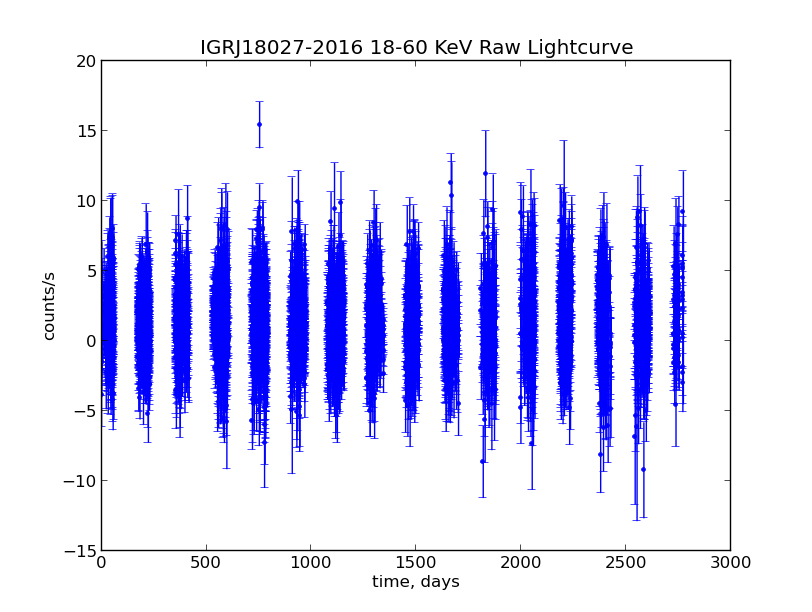
\includegraphics[width=130mm]{gfx/Fig1.png}
\caption{A raw lightcurve for the test source. Note the large errors on many data points.}
\label{Figure 1}
\end{figure}

\section{Re-binning the Data}
A simple tool for visualising the data is to be able to compile a graph of the entire light curve. However most sources from the archive have many thousands of individual science windows; the test source used had approximately 10,000. In order so that a sensible graph can be produced, the data shown needs to be cut down in a way that throws away as little useful information as possible. Re-binning collects groups of data points into a single data point. 

In the project code, a uniform bin size is selected, typically between 1 day to 1 month. Data points are grouped into the bins, and a flux measurement for each bin is calculated by taking an average of the members, weighted by the standard error. Furthermore, a new standard error is calculated for each bin by propagating errors through the calculation of the binned flux.

Re-binning the data is useful for visualising the data. However, a graph produced by re-binning the data will not show any variation in the source on a time period smaller than the bin size. Binning into one month bins loses all information that happens in the timescale of the orbital period of the object, which may be only a few days. This makes re-binning only a preliminary step in analysing a source. 

\begin{figure}[h!]
\centering
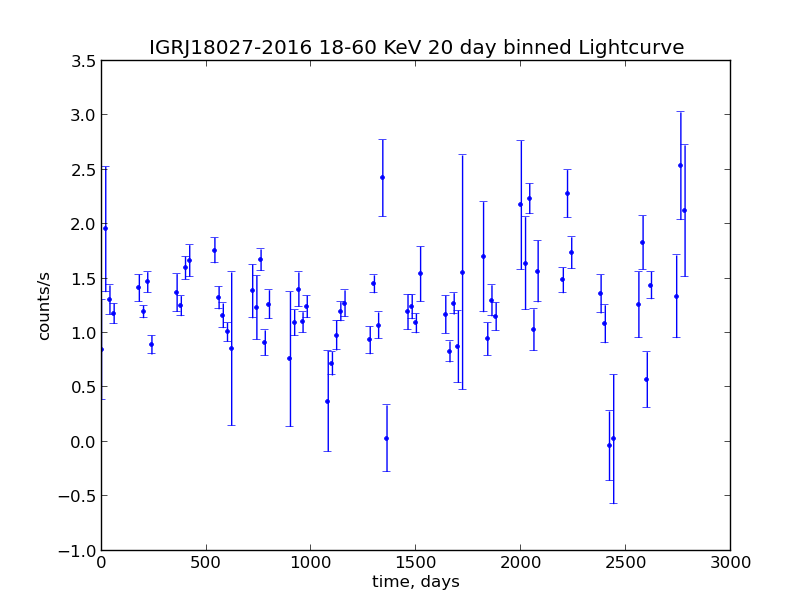
\includegraphics[width=130mm]{gfx/Fig2.png}
\caption{A re-binned light curve for the test source, with a 20 day bin size.}
\label{Figure 2}
\end{figure}

\ref{Figure 1} shows a raw lightcurve for the test source. Note the large errors on many data points. 
\ref{Figure 2} shows a re-binned light curve for the test source, with a 20 day bin size. Note that when only a few data points fall into a single bin, the bin can appear to have a large error. The points in the figure with the smallest error bars are typically calculated from many data points in the raw lightcurve.

\section{Finding Periodicities}
One of the key aims of the project is to find periodicities in the sample of sources, so it is necessary to have robust method to detect this within the data. One common method employed is to perform Fourier analysis. In breaking down the data into a series of sine waves, the periodic variations in flux will show up as the sine waves with the largest coefficients. However, Fourier analysis requires that the data points are evenly spaced, a criterion not often fulfilled in astronomy, and also not true of the INTEGRAL data.

\begin{figure}[h!]
\centering
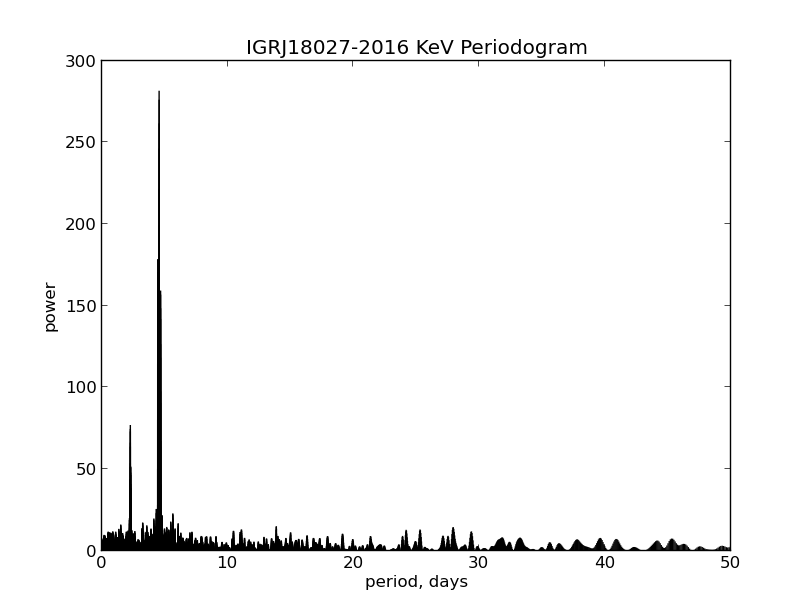
\includegraphics[width=130mm]{gfx/Fig3.png}
\caption{A periodogram for the test source, using the astropython implementation.}
\label{Figure 3}
\end{figure}

\subsection{Lomb-Scargle Method}
One alternative method, that this project uses, is the Lomb-Scargle method. This method fits trial sine waves to the data and then by minimising the squares of the residuals, produces a spectrum of the data. Crucially, the Lomb-Scargle Method can work on unevenly sampled data. 
There are two easily available implementations of the Lomb-Scargle method in python. One is available in Scipy 0.11 and another has been implemented by a contributor to astropython, which this project uses [ref]. Both implementations utilise Numpy, which has routines that are pre-compiled in C and Fortran, making the routine efficient.

Two useful outputs are produced from this section of the code. The first is the periodogram, which is a spectrum of the data. The test source is known to have a strong periodicity associated with an eclipse. This shows up clearly in the periodogram. Second, the Lomb-Scargle routine returns the highest peak in the periodogram, which corresponds to the strongest period. This is passed to the next section of the code for producing the folded light curves.

Whilst both routines perform the same overall function, the inner workings are a \textquotedblleft{}black box\textquotedblright{}. Experience showed that the astropython routine appeared to find a stronger peak, however there were exceptions where the Scipy implementation performed better. In general, the astropython implementation is shown, unless stated otherwise.

\begin{figure}[h!]
\centering
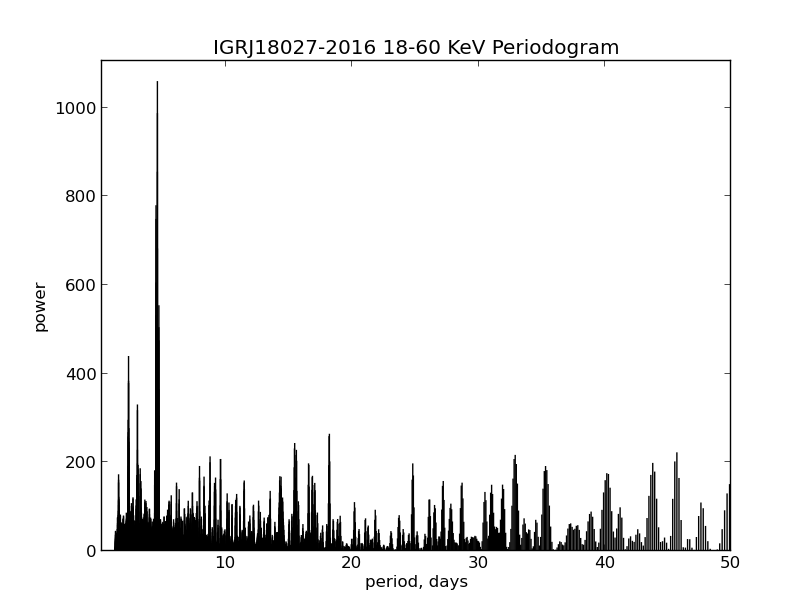
\includegraphics[width=130mm]{gfx/Fig4.png}
\caption{A periodogram for the test source, using the Scipy implementation.}
\label{Figure 4}
\end{figure}


\ref{Figure 3} shows a periodogram for the test source, using the astropython implementation. It shows a strong peak in power at approximately 4.6 days, which is due to the eclipse.
\ref{Figure 4} shows a periodogram for the test source, using the Scipy implementation. Whilst it also shows the same peak, it is obvious from inspection that the periodogram is more noisy.

\section{Folding the Lightcurve}
Using the period found from the Lomb-Scargle routine, the next step of the code is to produce a folded light curve. The light curve produced initially cannot reveal any significant amount of information about an object, since all variation is lost by re-binning the data. In the project code, by dividing each time coordinate by the period, and keeping only the remainder, the data is \textquotedblleft{}folded\textquotedblright{} on top of itself. This means that each identical point in the object\textquoteright{}s period will line up over each other. 

The next step is to define a set of bins, similar to the previous section, and to re-bin the folded data. Once again, a weighted average of the flux is taken, and errors calculated through. The number of bins is a trade-off. With a smaller number of bins, the averaging reduces the error on each measurement, however time resolution is lost. This can be seen in the test source, as each point of the eclipse occurs at the same place on the graph. Once averaged, the eclipse profile can be seen in the data, as the averaging process causes the points to converge to the true profile, and reduces the error greatly. 

\begin{figure}[h!]
\centering
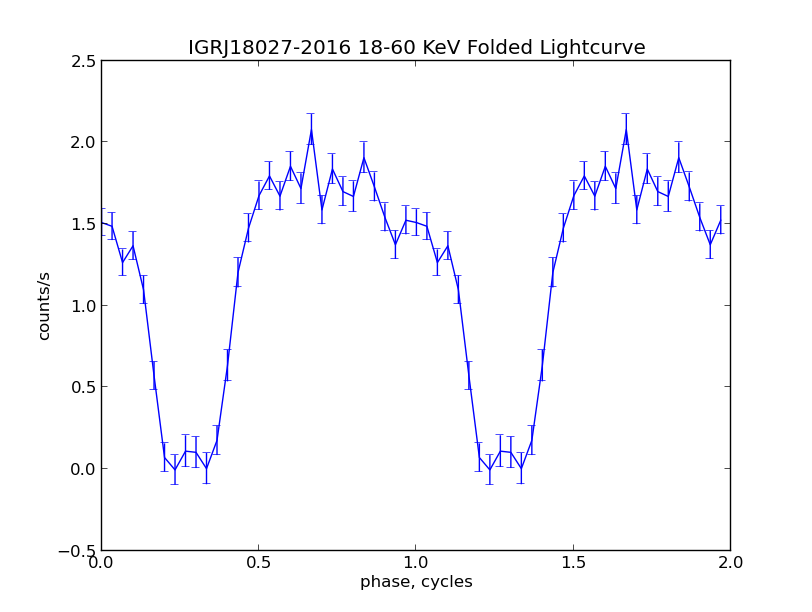
\includegraphics[width=130mm]{gfx/Fig5.png}
\caption{A folded and binned light curve, using the strongest peak from the periodogram, 4.570 days. Two cycles are shown for clarity.}
\label{Figure 5}
\end{figure}

\ref{Figure 5} shows the folded and binned light curve, using the strongest peak from the periodogram. Two cycles are shown for clarity. The eclipse shows through clearly, and the effect of the large data set reduces the size of the error bars significantly.

\subsection{Phase Dispersion Method}
Another means to detect periodicities in data is the Phase Dispersion Method. The Lomb-Scargle routine makes the implicit assumption that the signal in the data is sinusoidal, since all it fits are sine waves. This is a reasonable assumption when dealing with SGXBs such as the test source, and Cen X-3, since the eclipse is regular and the time of the eclipse forms a significant fraction of the folded light curve.  However, for sources such as BeXBs where the \textquotedblleft{}on time\textquotedblright{} of the sources is a very small fraction of the orbital period of the compact object, then this assumption breaks down. Sources that also have a high range, that flare particularly brightly also reduce the effectiveness of the Lomb-Scargle method. 
The Phase Dispersion Method makes no assumptions about the shape of the lightcurve. It works by attempting many trial folds of the data, and then binning the data down, where the process is the same that is used to produce the plot above. The key part of the method is that it compares the variance, or spread of points, within each bin to the variance of the entire data set as a whole. If a trial period is tested that is not a periodicity of the data, then the variance of points within a bin will on average be the same as the variance of the data as a whole. However if a trial period is tested that is a periodicity of the data, then the points within a bin will tend to cluster more tightly. This can be represented as a statistic for each trial fold, which tends to be $\simeq1$ for noise, and then reduces when a periodicity is found.

\begin{figure}[h!]
\centering
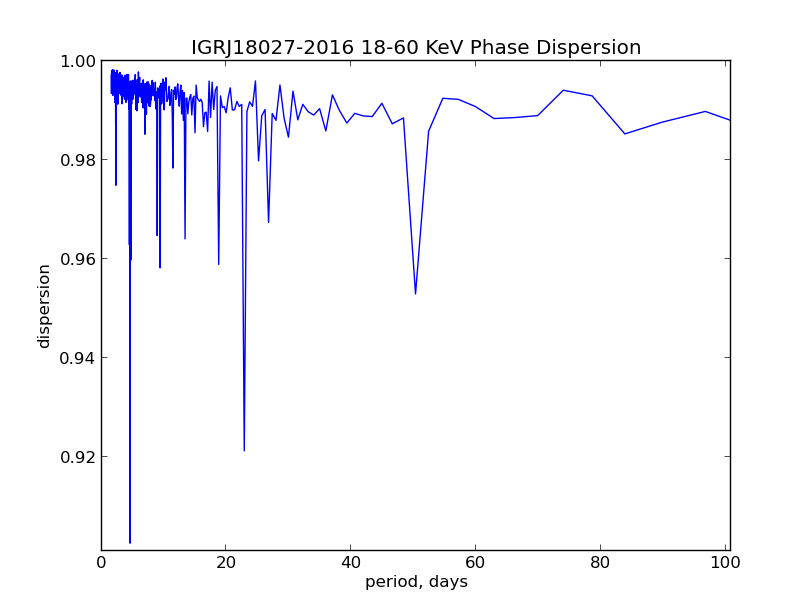
\includegraphics[width=130mm]{gfx/Fig6.png}
\caption{A PDM plot for the test source. Notice where the drop in the statistic coincides with the peak in the Lomb-Scargle periodogram, and the harmonics of the strongest frequency.}
\label{Figure 6}
\end{figure}

\ref{Figure 6} shows a PDM plot for the same test source. Notice where the drop in the statistic coincides with the peak in the Lomb-Scargle periodogram, and the harmonics of the strongest frequency.

Unfortunately, no PDM method already exists in any available python library, so this was coded from scratch. PAPER was used as a reference to code the method. This proved to be a technical challenge during the project. Furthermore, since the method is coded almost entirely in python, and due to the inherent nature of having to perform many trial folds of the data, the method is considerably slower to produce the same results as the Lomb-Scargle method. 

\section{Error calculations of the Lomb-Scargle Period}

When dealing with more challenging sources, it\textquoteright{}s useful to be able to quantify how accurate the period found by the Lomb-Scargle routine is. It\textquoteright{}s difficult to calculate errors conventionally, and also challenging to implement this in code. Two solutions were coded to be used in the project to find an error measurement. 

A Monte-Carlo simulation randomises the data. Each flux value is randomised according to a normal distribution with mean given by the flux and standard deviation given by its error. This generates a modified light curve which is processed by the Lomb-Scargle routine. The period is recorded, and the process repeated with a new randomised light curve generated from the original. Typically ten thousand runs are made as a minimum. A histogram of the periods is plotted, which should approximate a normal distribution with standard deviation that is the error on the original period.

Bootstrapping is another similar method. Rather than randomising the data, bootstrapping randomly discards data from the set. For N data points, N random integers between 1 and N are generated. Each integer corresponds to a data point, so that if the number X is generated, the Xth data point is copied to a new light curve. This allows for duplicate random integers, however the data point is only copied once. This reduced light curve is run through the routine, the period recorded, and a new light curve generated to repeat the process. 
